\documentclass[xcolor=dvipsnames, xcolor=table]{beamer} % Classe de documento para apresentações
\usepackage{listings}
\usepackage{listings}\usetheme{Berlin}
\usecolortheme{beaver}
\usepackage{textpos}
\usepackage{color}
\usepackage{wasysym}
\renewcommand\tabcolsep{4pt}
\usepackage{csquotes} 
\usepackage{wrapfig}
\usepackage{microtype}
\usepackage[labelfont=bf]{caption}
\usepackage{epigraph}
\usepackage[english]{babel}
\usepackage{float}
\usepackage{hyperref}
\usepackage{amsmath}
\newcommand{\dd}[1]{\mathrm{d}#1}
\usepackage{amsfonts}
\usepackage{amssymb}
\usepackage{amsbsy}
\usepackage{graphicx}
\usepackage{mathtools}

\usepackage{booktabs}

\usepackage{adjustbox}
\hypersetup{pdfpagemode=FullScreen} % para o pdf abrir automaticamente em modo full screen
\setbeamertemplate{caption}[numbered] % para numerar as tabelas
\usepackage{subcaption}
\usepackage[none]{hyphenat} 
\usepackage{bm} %%% bold vectors
\usepackage{tabularx}  
\usepackage{tikz}




\setbeamercolor{author in head/foot}{fg=Maroon}     % cor do nome do autor no rodape
\setbeamercolor{institute in head/foot}{fg=Maroon}  % cor do nome do ISEG no rodape
\setbeamercolor{frametitle}{fg=Maroon, bg=black!9} % cor da letra e do fundo fa faixa com o nome de cada slide
\setbeamercolor{caption name}{fg=Maroon, bg=black!9}
\setbeamercolor*{title}{fg=white, bg=Maroon}          % cor do titulo e da caixa de titulo na capa
\setbeamercolor{itemize item}{fg=Maroon}               % cor dos bullets do ambiente \itemize 


\makeatletter % criaçao de um ambiente sem TOC no cabeçalho do slide
\newenvironment{noheadline}{
\setbeamertemplate{headline}{}
\addtobeamertemplate{frametitle}{\vspace*{-0.9\baselineskip}}{}
}{}
\makeatother

\usepackage[beamer,customcolors]{hf-tikz}

\tikzset{hl/.style={
    set fill color=red!80!black!40,
    set border color=red!80!black,
  },
}


\title[Non-Numeric Values]{Non-Numeric Values}
\author[Pedro Fonseca]{\textbf {Pedro Fonseca}}
\titlegraphic{
\includegraphics[width=1.5cm]{yes}}
\institute[Introduction to R]{\textbf {Introduction to R}}
\date{\today}


% position the yes
\addtobeamertemplate{frametitle}{}{%
\begin{textblock*}{100mm}(.85\textwidth,-.9cm)

\includegraphics[scale=.05]{yes}
\end{textblock*}}



%%%%%%%%%%%%% Ambiente de teorema/definição com as cores do ISEG %%%%%%

\makeatletter
\def\th@mystyle{%
    \normalfont % body font
    \setbeamercolor{block title example}{bg=Maroon,fg=white}
    \setbeamercolor{block body example}{bg=black!9,fg=black}
    \def\inserttheoremblockenv{exampleblock}
  }
\makeatother
\theoremstyle{mystyle}
\newtheorem*{defi}{Definição}

\setbeamertemplate{defis}[numbered]



%%%%%%%%%%%%%%%% Bibliografia %%%%%%%%%%%%%%%%%%%%%%%

\usepackage{url}
\usepackage[style=authoryear, bibencoding=utf8, minnames=1, maxnames=3,
maxbibnames=99,backref=true, natbib=true, dashed=false, terseinits=true, 
firstinits=true, uniquename=false, uniquelist=true, labeldate=true, 
doi=false, isbn=false, natbib=true, backend=biber]{biblatex}
\DefineBibliographyStrings{english}{%
    backrefpage = {Cited on page},
    backrefpages = {Cited on pages},
}
% Change the default formatting to be more "statistical"
\DeclareFieldFormat{url}{\url{#1}}
\DeclareFieldFormat[article]{pages}{#1}
\DeclareFieldFormat[inproceedings]{pages}{\lowercase{pp.}#1}
\DeclareFieldFormat[incollection]{pages}{\lowercase{pp.}#1}
\DeclareFieldFormat[article]{volume}{\mkbibbold{#1}}
\DeclareFieldFormat[article]{number}{\mkbibparens{#1}}
\DeclareFieldFormat[article]{title}{\MakeCapital{#1}}
\DeclareFieldFormat[article]{url}{}
\DeclareFieldFormat[book]{url}{}
\DeclareFieldFormat[inbook]{url}{}
\DeclareFieldFormat[incollection]{url}{}
\DeclareFieldFormat[inproceedings]{url}{}
\DeclareFieldFormat[inproceedings]{title}{#1}
\DeclareFieldFormat{shorthandwidth}{#1}
% No dot before number of articles
\usepackage{xpatch}
\xpatchbibmacro{volume+number+eid}{\setunit*{\adddot}}{}{}{}
% Remove In: for an article.
\renewbibmacro{in:}{%
  \ifentrytype{article}{}{%
  \printtext{\bibstring{in}\intitlepunct}}}
% Get rid of months in citations
\AtEveryBibitem{\clearfield{month}}
\AtEveryCitekey{\clearfield{month}}
\setlength{\parindent}{1,3cm}
\raggedbottom

\renewcommand\bibfont{\scriptsize}
% If you have more than one page of references, you want to tell beamer
% to put the continuation section label from the second slide onwards
\setbeamertemplate{frametitle continuation}[from second]
% Now get rid of all the colours
\setbeamercolor*{bibliography entry title}{fg=black}
\setbeamercolor*{bibliography entry author}{fg=black}
\setbeamercolor*{bibliography entry location}{fg=black}
\setbeamercolor*{bibliography entry note}{fg=black}





\begin{document}
%%%%%%%%%%%%%%%%%%%%%  CAPA  %%%%%%%%%%%%%%%%%%%%%%%%%%%%%
\begin{noheadline}

\begin{frame}%[plain]
\vfill
\centering

\begin{beamercolorbox}[sep=8pt,center,colsep=-4bp,rounded=true,shadow=true]{title}
\usebeamerfont{title}\inserttitle\par%
\ifx\insertsubtitle\@empty%
\else%
\vskip0.25em%
{\usebeamerfont{subtitle}\usebeamercolor[fg]{subtitle}\insertsubtitle\par}%
\fi%     
\end{beamercolorbox}%

\vskip1em\par

\begin{beamercolorbox}[sep=8pt,center,colsep=-4bp,rounded=true,shadow=true]{author}
\usebeamerfont{author}\insertauthor
\end{beamercolorbox}

{\usebeamercolor[fg]{titlegraphic}\inserttitlegraphic\par}

\begin{beamercolorbox}[sep=8pt,center,colsep=-4bp,rounded=true,shadow=true]{institute}
\usebeamerfont{institute}\insertinstitute
\end{beamercolorbox}

\begin{beamercolorbox}[sep=8pt,center,colsep=-4bp,rounded=true,shadow=true]{date}
\usebeamerfont{date}\insertdate
\end{beamercolorbox}\vskip0.5em

\end{frame}
\end{noheadline}



%%%%%%%%%%%%%% ITEMIZE SHAPES AND COLLERS%%%%%%%%%%%%%%%%%%%%%%%%%

\setbeamertemplate{itemize item}{\color{Maroon}\newmoon}
\setbeamertemplate{itemize subitem}{\color{Maroon}$\blacktriangleright$}



%%%%%%%%%%%%%%%%%%%%%%%%%%%%%%%%%%%%%%%%%%%%%%%%%%%%%%%%%%%%%%%

\section{Logical values}  

\subsection{Logical Values and Logical Operations}

\begin{frame}[fragile] %%%%%%%%%%%%%%%%%%%%%%% FRAME %%%%%%%%%%%%%%%%%%%%%%%%%%%%
\frametitle{Introduction}
\begin{itemize}
\item Statistical programming sometimes requires non-numeric values. 
\item Examples of non numerical values in R: characters and logical values. 
\end{itemize}

\end{frame}



\begin{frame}[fragile] %%%%%%%%%%%%%%%%%%%%%%% FRAME %%%%%%%%%%%%%%%%%%%%%%%%%%%%
\frametitle{What are logical values?}
\begin{itemize}
\item Logical values can only have two values: TRUE or FALSE.
\item Logical values in R can be abbreviated as T or F.

\begin{verbatim}
> foo <- TRUE
> foo
[1] TRUE

> bar <- F
> bar
[1] FALSE
\end{verbatim}
\end{itemize}
\end{frame}

\begin{frame}[fragile] %%%%%%%%%%%%%%%%%%%%%%% FRAME %%%%%%%%%%%%%%%%%%%%%%%%%%%%

\frametitle{Logical vectors and matrices}

\begin{itemize}

\item A logical vector:

\begin{verbatim}
> baz <- c(TRUE, FALSE, FALSE, FALSE, TRUE, FALSE)
> baz
[1]  TRUE FALSE FALSE FALSE  TRUE FALSE
\end{verbatim}

\item A logical  matrix: 

\begin{verbatim}
> qux <- matrix(data = baz, nrow = 3, ncol = 2)
> qux
      [,1]  [,2]
[1,]  TRUE FALSE
[2,] FALSE  TRUE
[3,] FALSE FALSE
\end{verbatim}

\end{itemize}


\end{frame}

\begin{frame}[fragile] %%%%%%%%%%%%%%%%%%%%%%% FRAME %%%%%%%%%%%%%%%%%%%%%%%%%%%%
\frametitle{Basic logical operators}

\begin{figure}[H]
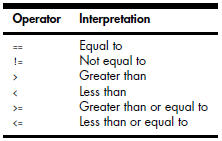
\includegraphics[width=7.5cm]{Screenshot_1}
\caption{Basic logical operators in R}
\end{figure}

\end{frame}



\begin{frame}[fragile] %%%%%%%%%%%%%%%%%%%%%%% FRAME %%%%%%%%%%%%%%%%%%%%%%%%%%%%

\frametitle{Logical comparisons}

\begin{itemize}
\item Logicals can be used to check relationships between values:
\begin{verbatim}
> 1 == 2
[1] FALSE

> 1>2
[1] FALSE

> (2-1) <= 2
[1] TRUE

> 1 != (2+3)
[1] TRUE

\end{verbatim}
\end{itemize}
\end{frame}

\begin{frame}[fragile] %%%%%%%%%%%%%%%%%%%%%%% FRAME %%%%%%%%%%%%%%%%%%%%%%%%%%%%

\frametitle{Logical comparisons}

\begin{itemize}
\item Logicals can be used to check relationships between variables:
\begin{verbatim}

> x <- log(5, base = 10)
> y <- log(5, base = exp(1))

> y == x
[1] FALSE
> y >= x
[1] TRUE

> c(x, y)
[1] 0.698970 1.609438

\end{verbatim}
\end{itemize}
\end{frame}

\begin{frame}[fragile] %%%%%%%%%%%%%%%%%%%%%%% FRAME %%%%%%%%%%%%%%%%%%%%%%%%%%%%

\frametitle{Vectorized logical comparison}


\begin{verbatim}

> vec_x <- c(1, 5, 6, 7, 3)
> vec_y <- c(1, 6, 8, 2, 1)

> vec_x == 5
[1] FALSE  TRUE FALSE FALSE FALSE
> vec_x != 5
[1]  TRUE FALSE  TRUE  TRUE  TRUE
> vec_x >= vec_y
[1]  TRUE FALSE FALSE  TRUE  TRUE

\end{verbatim}
\end{frame}

\begin{frame}[fragile] %%%%%%%%%%%%%%%%%%%%%%% FRAME %%%%%%%%%%%%%%%%%%%%%%%%%%%%

\frametitle{The ! operator}

\begin{itemize}
\item "!" is the negation (NOT) operator
\begin{verbatim}

> !TRUE
[1] FALSE

> !FALSE
[1] TRUE

> !c(TRUE, FALSE, TRUE, TRUE, FALSE)
[1] FALSE  TRUE FALSE FALSE  TRUE

\end{verbatim}
\end{itemize}
\end{frame}

\begin{frame}[fragile] %%%%%%%%%%%%%%%%%%%%%%% FRAME %%%%%%%%%%%%%%%%%%%%%%%%%%%%

\frametitle{The ! operator}

\begin{verbatim}

> x <- c(FALSE, TRUE)
> !x
[1]  TRUE FALSE

\end{verbatim}
\end{frame}

\begin{frame}[fragile] %%%%%%%%%%%%%%%%%%%%%%% FRAME %%%%%%%%%%%%%%%%%%%%%%%%%%%%

\frametitle{The ! operator}


\begin{verbatim}

> vec_x <- c(1, 5, 6, 7, 3)
> vec_y <- c(1, 6, 8, 2, 1)

> vec_x >= vec_y
[1]  TRUE FALSE FALSE  TRUE  TRUE

> !(vec_x >= vec_y)
[1] FALSE  TRUE  TRUE FALSE FALSE

\end{verbatim}
\end{frame}

\begin{frame}[fragile] %%%%%%%%%%%%%%%%%%%%%%% FRAME %%%%%%%%%%%%%%%%%%%%%%%%%%%%

\frametitle{The ! operator}

\begin{verbatim}

> vec_x <- c(1, 5, 6, 7, 3)
> vec_y <- c(1, 6, 8, 2, 1)

> vec_x == 5
[1] FALSE  TRUE FALSE FALSE FALSE
> !(vec_x == 5)
[1]  TRUE FALSE  TRUE  TRUE  TRUE

> vec_x == vec_y
[1]  TRUE FALSE FALSE FALSE FALSE

\end{verbatim}
\end{frame}

\begin{frame}[fragile] %%%%%%%%%%%%%%%%%%%%%%% FRAME %%%%%%%%%%%%%%%%%%%%%%%%%%%%

\frametitle{! vs \textit{Factorial}}

\begin{itemize}
\item Do not confuse "!" with the factorial function
\item In R, the factorial function is \textit{factorial}:

\begin{verbatim}
> factorial(5)
[1] 120
> 5 * 4 * 3 * 2 * 1
[1] 120
\end{verbatim}

\item Alternatively, can use the product function:
\begin{verbatim}
> prod(5:1)
[1] 120
> prod(5, 4, 3, 2, 1)
[1] 120

\end{verbatim}
\end{itemize}


\end{frame}

\subsection{Subseting and Overwriting with Logicals}

\begin{frame}[fragile] %%%%%%%%%%%%%%%%%%%%%%% FRAME %%%%%%%%%%%%%%%%%%%%%%%%%%%%
\frametitle{Subset with logicals}

\begin{verbatim}
> myvec <- c(5, -2.3, 4, 4, 1)

> myvec[c(TRUE, FALSE, TRUE, FALSE, FALSE)]
[1] 5 4
\end{verbatim}

\begin{itemize}
\item Recycling rules apply as usual:

\begin{verbatim}
> myvec[c(TRUE, FALSE)]
[1] 5 4 1
\end{verbatim}
\end{itemize}

\end{frame}

\begin{frame}[fragile] %%%%%%%%%%%%%%%%%%%%%%% FRAME %%%%%%%%%%%%%%%%%%%%%%%%%%%%
\frametitle{Subset with logicals}

\begin{verbatim}
> mymat <- matrix(1:9, nrow = 3)
> mymat
     [,1] [,2] [,3]
[1,]    1    4    7
[2,]    2    5    8
[3,]    3    6    9

> mymat[, c(TRUE, FALSE, TRUE)]
     [,1] [,2]
[1,]    1    7
[2,]    2    8
[3,]    3    9

\end{verbatim}

\end{frame}

\begin{frame}[fragile] %%%%%%%%%%%%%%%%%%%%%%% FRAME %%%%%%%%%%%%%%%%%%%%%%%%%%%%
\frametitle{Subset with logicals}

\begin{verbatim}

> mymat[c(TRUE, TRUE, FALSE), ]
     [,1] [,2] [,3]
[1,]    1    4    7
[2,]    2    5    8

> mymat[c(TRUE, TRUE, FALSE), c(TRUE, TRUE, FALSE)]
     [,1] [,2]
[1,]    1    4
[2,]    2    5
\end{verbatim}

\end{frame}

\begin{frame}[fragile] %%%%%%%%%%%%%%%%%%%%%%% FRAME %%%%%%%%%%%%%%%%%%%%%%%%%%%%

\frametitle{Subset with logicals}

\begin{verbatim}
> myvec <- c(5, -2.3, 4, 4, -1)
 
> myvec < 0
[1] FALSE  TRUE FALSE FALSE  TRUE
> myvec[myvec < 0]
[1] -2.3 -1.0
 
> myvec != 4
[1]  TRUE  TRUE FALSE FALSE  TRUE
> myvec[myvec != 4]
[1]  5.0 -2.3 -1.0
\end{verbatim}

\end{frame}

\begin{frame}[fragile] %%%%%%%%%%%%%%%%%%%%%%% FRAME %%%%%%%%%%%%%%%%%%%%%%%%%%%%

\frametitle{Overwriting with logicals}

\begin{verbatim}
> mymat <- matrix(1:9, nrow = 3, byrow = TRUE)
> mymat
     [,1] [,2] [,3]
[1,]    1    2    3
[2,]    4    5    6
[3,]    7    8    9

> mymat < 5
      [,1]  [,2]  [,3]
[1,]  TRUE  TRUE  TRUE
[2,]  TRUE FALSE FALSE
[3,] FALSE FALSE FALSE
\end{verbatim}

\end{frame}

\begin{frame}[fragile] %%%%%%%%%%%%%%%%%%%%%%% FRAME %%%%%%%%%%%%%%%%%%%%%%%%%%%%

\frametitle{Overwriting with logicals}

\begin{verbatim}
> mymat[mymat < 5]
[1] 1 4 2 3

> mymat[mymat < 5] <- 0
> mymat
     [,1] [,2] [,3]
[1,]    0    0    0
[2,]    0    5    6
[3,]    7    8    9
\end{verbatim}

\end{frame}

\begin{frame}[fragile] %%%%%%%%%%%%%%%%%%%%%%% FRAME %%%%%%%%%%%%%%%%%%%%%%%%%%%%

\frametitle{Overwriting with logicals}

\begin{verbatim}
> mymat <- matrix(1:9, nrow = 3, byrow = TRUE)
> mymat
     [,1] [,2] [,3]
[1,]    1    2    3
[2,]    4    5    6
[3,]    7    8    9

> which(mymat < 5)
[1] 1 2 4 7

> mymat[which(mymat < 5)] <- 0 # same result as the  
>   								   # previous slide
\end{verbatim}

\end{frame}

\subsection{Missing Values}

\begin{frame}[fragile] %%%%%%%%%%%%%%%%%%%%%%% FRAME %%%%%%%%%%%%%%%%%%%%%%%%%%%%

\frametitle{Introduction}

\begin{itemize}
\item In R, missing values are represented by NA (not available)
\item NAs are exceptional logical values.
\item The \textit{is.logical} testes whether or not values are logic:

\begin{verbatim}
> is.logical(54)
[1] FALSE
> is.logical(myvec)
[1] FALSE
> is.logical(TRUE)
[1] TRUE
> is.logical(FALSE)
[1] TRUE
> is.logical(NA)
[1] TRUE
\end{verbatim}

\end{itemize}

\end{frame}

\begin{frame}[fragile] %%%%%%%%%%%%%%%%%%%%%%% FRAME %%%%%%%%%%%%%%%%%%%%%%%%%%%%

\frametitle{Introduction}

\begin{itemize}
\item In the previous lesson, we dealt with numerical values
\item There is also a test function for numerics:

\begin{verbatim}
> is.numeric(54)
[1] TRUE
> is.numeric(myvec)
[1] TRUE
> is.numeric(TRUE)
[1] FALSE
> is.numeric(FALSE)
[1] FALSE
> is.numeric(NA)
[1] FALSE
\end{verbatim}

\end{itemize}

\end{frame}

\begin{frame}[fragile] %%%%%%%%%%%%%%%%%%%%%%% FRAME %%%%%%%%%%%%%%%%%%%%%%%%%%%%

\frametitle{Operations with NAs}

\begin{itemize}
\item When NAs are present, caution is required!

\begin{verbatim}
> y <- c(1, 2, 3, NA)

> NA + 5
[1] NA
 > (NA + 3) > 0
[1] NA

> sum(1, 5, 6, NA, 7)
[1] NA 
> mean(y)
[1] NA
\end{verbatim}

\end{itemize}

\end{frame}

\begin{frame}[fragile]

\begin{itemize}
\frametitle{Dealing with missing values}
\item Many functions have a \textit{na.rm} argument. It is set to FALSE by default. 

\begin{verbatim}
> y <- c(1, 2, 3, 7, 0.5, NA)
> y_without_nas <- y[-6]

> mean(y, na.rm = TRUE)
[1] 2.7
> mean(y_without_nas)
[1] 2.7
> sum(1, 5, 6, NA, 7, na.rm = TRUE)
[1] 19
> sum(1, 5, 6, 7)
[1] 19
\end{verbatim}

\end{itemize}

\end{frame}

\begin{frame}[fragile]

\begin{itemize}
\frametitle{Dealing with missing values}
\item Other option: \textit{na.omit}

\begin{verbatim}
> y <- c(1, 2, 3, 7, 0.5, NA)
> na.omit(y)
[1] 1.0 2.0 3.0 7.0 0.5

> y_new <- na.omit(y)
> y_new
[1] 1.0 2.0 3.0 7.0 0.5
\end{verbatim}

\end{itemize}

\end{frame}

\begin{frame}[fragile]

\begin{itemize}
\frametitle{Dealing with missing values}
\item  \textit{na.omit} with matrices:

\begin{verbatim}
> (M <- matrix(c(1:3, NA, c(5, 9)), nrow = 3,
 byrow = TRUE))
     [,1] [,2]
[1,]    1    2
[2,]    3   NA
[3,]    5    9
> 
> na.omit(M)
     [,1] [,2]
[1,]    1    2
[2,]    5    9
\end{verbatim}

\end{itemize}

\end{frame}

\begin{frame}
\begin{itemize}
\frametitle{Dealing with missing values}
\item  In matrices (and data frames) \textit{na.omit} returns only complete rows!
\item This can be useful in data analysis when only complete cases are to be considered.
\item However, sometimes we have small samples and can't afford to throw away incomplete observations. 
\begin{itemize}
\item Solution: imputation
\end{itemize}
\end{itemize}
\end{frame}

\begin{frame}[fragile] %%%%%%%%%%%%%%%%%%%%%%% FRAME %%%%%%%%%%%%%%%%%%%%%%%%%%%%

\frametitle{Testing for missing values}


\begin{verbatim}
> y <- c(1, 2 , 3, NA)

> is.na(y)
[1] FALSE FALSE FALSE  TRUE

> !is.na(y)
[1]  TRUE  TRUE  TRUE FALSE
\end{verbatim}


\end{frame}

\begin{frame}[fragile] %%%%%%%%%%%%%%%%%%%%%%% FRAME %%%%%%%%%%%%%%%%%%%%%%%%%%%%

\frametitle{Testing for missing values}

\begin{verbatim}
> M <- matrix(c(1:3, NA, c(5, 9)), 3, 2, TRUE)
> M
     [,1] [,2]
[1,]    1    2
[2,]    3   NA
[3,]    5    9

> is.na(M)
      [,1]  [,2]
[1,] FALSE FALSE
[2,] FALSE  TRUE
[3,] FALSE FALSE
\end{verbatim}

\end{frame}

\begin{frame}[fragile] %%%%%%%%%%%%%%%%%%%%%%% FRAME %%%%%%%%%%%%%%%%%%%%%%%%%%%%

\frametitle{Imputation of missing values}

\begin{verbatim}
> M <- matrix(c(1:3, NA, c(5, NA)), 2, 3, TRUE)
> M
     [,1] [,2] [,3]
[1,]    1    2    3
[2,]   NA    5   NA

> is.na(M)
      [,1]  [,2]  [,3]
[1,] FALSE FALSE FALSE
[2,]  TRUE FALSE  TRUE

\end{verbatim}

\end{frame}

\begin{frame}[fragile] %%%%%%%%%%%%%%%%%%%%%%% FRAME %%%%%%%%%%%%%%%%%%%%%%%%%%%%

\frametitle{Imputation of missing values}

\begin{verbatim}
> M[is.na(M)] <- 0
> M

     [,1] [,2] [,3]
[1,]    1    2    3
[2,]    0    5    0
\end{verbatim}

\begin{itemize}
\item Replacing missing values with zeros can result in severe underestimation of the actual values. Sometimes it better to replace NAs with an estimate of its value.
\end{itemize}

\end{frame}

\begin{frame}[fragile] %%%%%%%%%%%%%%%%%%%%%%% FRAME %%%%%%%%%%%%%%%%%%%%%%%%%%%%

\frametitle{Imputation of missing values}

\begin{verbatim} 
> M <- cbind(
   y  = c(3, NA, 7, 1),
   x1 = c(1, 7,  9, 6),
   x2 = c(6, 7,  9, NA)
 )

> M
      y x1 x2
[1,]  3  1  6
[2,] NA  7  7
[3,]  7  9  9
[4,]  1  6 NA
\end{verbatim}

\end{frame}

\begin{frame}[fragile] %%%%%%%%%%%%%%%%%%%%%%% FRAME %%%%%%%%%%%%%%%%%%%%%%%%%%%%

\frametitle{Imputation of missing values}

\begin{verbatim} 
> M[, "y"]
[1]  3 NA  7  1

> is.na(M[, "y"])
[1] FALSE  TRUE FALSE FALSE

> M[is.na(M[, "y"]), "y"] <- median(M[, "y"],
 na.rm = TRUE)

> M[is.na(M[, "x2"]), "x2"] <- median(M[, "x2"],
 na.rm = TRUE)

\end{verbatim}

\end{frame}

\begin{frame}[fragile] %%%%%%%%%%%%%%%%%%%%%%% FRAME %%%%%%%%%%%%%%%%%%%%%%%%%%%%

\frametitle{Imputation of missing values}

\begin{verbatim} 

> M
     y x1 x2
[1,] 3  1  6
[2,] 3  7  7
[3,] 7  9  9
[4,] 1  6  7
\end{verbatim}

\end{frame}

\begin{frame}[fragile] %%%%%%%%%%%%%%%%%%%%%%% FRAME %%%%%%%%%%%%%%%%%%%%%%%%%%%%
\frametitle{Counting missing values}

\begin{itemize}
\item The \textit{table} function is useful here:
\begin{verbatim}
> y <- c(1, 2 , 3, NA, 6, NA, 9, NA)

> is.na(y)
[1] FALSE FALSE FALSE  TRUE FALSE  TRUE FALSE  TRUE

> table(is.na(y))
FALSE  TRUE 
    5     3 
\end{verbatim}
\end{itemize}

\end{frame}

\begin{frame}[fragile] %%%%%%%%%%%%%%%%%%%%%%% FRAME %%%%%%%%%%%%%%%%%%%%%%%%%%%%
\frametitle{Counting missing values}

\begin{itemize}
\item  \textit{table} also works with matrices:
\begin{verbatim}
> M <- rbind(
   col1 <- c(2, 5, 7),
   col2 <- c(NA, 5, 7),
   col3 <- c(2, 5, NA)
  )

> table(is.na(M))

FALSE  TRUE 
    7     2 
\end{verbatim}
\end{itemize}

\end{frame}

\begin{frame}[fragile] %%%%%%%%%%%%%%%%%%%%%%% FRAME %%%%%%%%%%%%%%%%%%%%%%%%%%%%
\frametitle{Counting missing values}

\begin{itemize}
\item  Alternative: 
\begin{verbatim}
> y <- c(1, 2 , 3, NA, 6, NA, 9, NA)
> sum(is.na(y))
[1] 3

> M <- rbind(
   col1 <- c(2, 5, 7),
   col2 <- c(NA, 5, 7),
   col3 <- c(2, 5, NA)
 )
> sum(is.na(M))
[1] 2
\end{verbatim}
\end{itemize}

\end{frame}

\begin{frame}[fragile] %%%%%%%%%%%%%%%%%%%%%%% FRAME %%%%%%%%%%%%%%%%%%%%%%%%%%%%
\frametitle{Coercion of logical values}

\begin{itemize}
\item  Why does \textit{sum(is.na())} Work? R coerces logical values to numerical values if you use them in a context where numeric values are expected.

\item How?

\begin{verbatim}
> as.numeric(TRUE)
[1] 1
> as.numeric(FALSE)
[1] 0
\end{verbatim}

\item The \textit{as.numeric} function forces the coercion to numeric.

\end{itemize}

\end{frame}

\begin{frame}[fragile] %%%%%%%%%%%%%%%%%%%%%%% FRAME %%%%%%%%%%%%%%%%%%%%%%%%%%%%
\frametitle{Coercion of logical values}

\begin{verbatim}
> y <- c(1, 2 , 3, NA, 6, NA, 9, NA)
> is.na(y)
[1] FALSE FALSE FALSE  TRUE FALSE  TRUE FALSE  TRUE
> as.numeric(is.na(y))
[1] 0 0 0 1 0 1 0 1
> sum(as.numeric(is.na(y)))
[1] 3
\end{verbatim}
\begin{itemize}

\item The \textit{as.numeric} function here is redundant since R coerces the inputs of \textit{sum} to numerical if possible.
\item The same happens with matrices.
\end{itemize}

\end{frame}

\begin{frame}[fragile] %%%%%%%%%%%%%%%%%%%%%%% FRAME %%%%%%%%%%%%%%%%%%%%%%%%%%%%
\frametitle{Removing NAs with the \textit{which} function}

\begin{verbatim}
> y <- c(1, 2 , 3, NA, 6, NA, 9, NA)
\end{verbatim}

\begin{itemize}

\item How many NAs in y?

\begin{verbatim}
> length(which(is.na(y)))
[1] 3
\end{verbatim}

\item In which positions are the positions with non-NA values of y?

\begin{verbatim}
> which(is.na(y)) 
[1] 4 6 8
\end{verbatim}

\item Subset y to extract non-missing values only:

\begin{verbatim}
> y[which(!is.na(y))] # notice the "!"
[1] 1 2 3 6 9            
\end{verbatim}
\end{itemize}

\end{frame}

\subsection{Logical Comparisons with Multiple Conditions}

\begin{frame}[fragile] %%%%%%%%%%%%%%%%%%%%%%% FRAME %%%%%%%%%%%%%%%%%%%%%%%%%%%%
\frametitle{Logical comparison with more than one condition}

\begin{figure}[H]
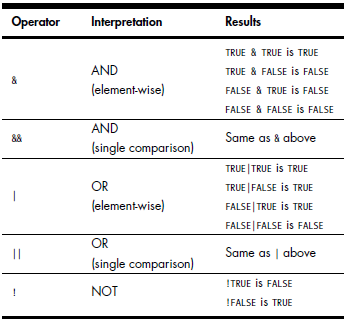
\includegraphics[scale = .6]{Screenshot_2}
\caption{The "and", "or" and "not" operators in R}
\end{figure}

\end{frame}

\begin{frame}[fragile] %%%%%%%%%%%%%%%%%%%%%%% FRAME %%%%%%%%%%%%%%%%%%%%%%%%%%%%
\frametitle{Logical comparison with more than one condition}

\begin{itemize}

\item Examples:

\begin{verbatim}
> (6 < 4) || (3 != 1)
[1] TRUE

> (6 < 4) || (3 == 1)
[1] FALSE

> (6 < 4) && (3 != 1)
[1] FALSE

> (6 > 4) && (3 >= 1)
[1] TRUE

\end{verbatim}

\end{itemize}

\end{frame}

\begin{frame}[fragile] %%%%%%%%%%%%%%%%%%%%%%% FRAME %%%%%%%%%%%%%%%%%%%%%%%%%%%%
\frametitle{Logical comparison with more than one condition}

\begin{itemize}

\item Examples:

\begin{verbatim}
> y <- c(1, 5 ,3, 1, 2, 9)

> (y > 2) & (y < 6)
[1] FALSE  TRUE  TRUE FALSE FALSE FALSE
 
> (y > 2) | (y < 6)
[1] TRUE TRUE TRUE TRUE TRUE TRUE

\end{verbatim}

\end{itemize}

\end{frame}

\begin{frame}[fragile] %%%%%%%%%%%%%%%%%%%%%%% FRAME %%%%%%%%%%%%%%%%%%%%%%%%%%%%
\frametitle{Logical comparison with more than one condition}

\begin{itemize}

\item Examples:

\begin{verbatim}
> y <- c(1, 5 ,3, 1, 2, 9)

> y[(y > 2) & (y < 6)]
[1] 5 3

> y[(y > 2) | (y < 6)]
[1] 1 5 3 1 2 9

\end{verbatim}

\end{itemize}

\end{frame}

\begin{frame}[fragile] %%%%%%%%%%%%%%%%%%%%%%% FRAME %%%%%%%%%%%%%%%%%%%%%%%%%%%%
\frametitle{Logical comparison with more than one condition}

\begin{itemize}

\item You can  chain as many comparisons as you want:

\begin{verbatim}
> y[y > 2]
[1] 5 3 9

> y[(y > 2) | (y < 6)]
[1] 1 5 3 1 2 9

> y[((y > 2) | (y < 6)) & (y != 2)]
[1] 1 5 3 1 9
\end{verbatim}

\item When performing multiple comparisons, parentheses are recommended!

\end{itemize}

\end{frame}

\begin{frame}[fragile] %%%%%%%%%%%%%%%%%%%%%%% FRAME %%%%%%%%%%%%%%%%%%%%%%%%%%%%
\frametitle{The \textit{any} and \textit{all} functions}

\begin{itemize}
\item Given a set of logical vectors, is at least one of the values true?
\item Given a set of logical vectors, are all of the values true?
\end{itemize}

\begin{verbatim}
> y <- c(1, 5 , 3, NA, 2, 9)

> any(y > 2, y < 6, !is.na(y))
[1] TRUE

> all(y > 2, y < 6, !is.na(y))
[1] FALSE
\end{verbatim}

\end{frame}

\begin{frame}[fragile] %%%%%%%%%%%%%%%%%%%%%%% FRAME %%%%%%%%%%%%%%%%%%%%%%%%%%%%
\frametitle{Exclusive OR}

\begin{itemize}
\item \textit{xor} indicates element-wise exclusive OR
\begin{verbatim}
> y <- c(1, 5 ,3, 1, 2, 9)

> xor(y>2, y<6)
[1]  TRUE FALSE FALSE  TRUE  TRUE  TRUE
\end{verbatim}

\end{itemize}

\end{frame}

\begin{frame}[fragile] %%%%%%%%%%%%%%%%%%%%%%% FRAME %%%%%%%%%%%%%%%%%%%%%%%%%%%%
\frametitle{Logical comparison with more than one condition}

\begin{figure}
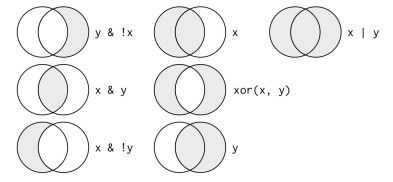
\includegraphics[scale=.8]{logical.png}
\caption{A visual perspective of logical operators}
\end{figure}

\end{frame}

\section{Characters}

\subsection{Introduction}

\begin{frame}[fragile] %%%%%%%%%%%%%%%%%%%%%%% FRAME %%%%%%%%%%%%%%%%%%%%%
\frametitle{Creating character values}

\begin{itemize}
\item Character strings are used to represent text, and should be inside single or double quotes:

\begin{verbatim}
> foo <- "hello world"
> foo
[1] "hello world"

> foo2 <- 'hello world'
> foo2
[1] "hello world"

\end{verbatim}
\end{itemize}
\end{frame}

\begin{frame}[fragile] %%%%%%%%%%%%%%%%%%%%%%% FRAME %%%%%%%%%%%%%%%%%%%%%
\frametitle{Basic functions for characters}

\begin{itemize}
\item Character strings are used to represent text, and should be inside single or double quotes:

\begin{verbatim}
> foo <- "hello world"
> foo
[1] "hello world"

> length(foo)
[1] 1

> nchar(foo)
[1] 11
\end{verbatim}
\end{itemize}
\end{frame}

\begin{frame}
\frametitle{Common use of characters in R}

\begin{itemize}
\item Provide arguments to functions
\item Directories
\item Create factors
\item Create names (vectors, matrices, lists, data frames)
\end{itemize}
\end{frame}

\begin{frame}[fragile] %%%%%%%%%%%%%%%%%%%%%%% FRAME %%%%%%%%%%%%%%%%%%%%%
\frametitle{Introduction}

\begin{itemize}

\item When writing strings, you can insert single quotes in a string with double quotes, and vice versa:

\begin{verbatim}
# single quotes within double quotes
ex1 <- "The 'R' project for statistical computing"

# double quotes within single quotes
ex2 <- 'The "R" project for statistical computing'
\end{verbatim}

\item You cannot directly insert single quotes in a string with single quotes, neither you can insert double quotes in a string with double quotes

\end{itemize}
\end{frame}

\begin{frame}[fragile] %%%%%%%%%%%%%%%%%%%%%%% FRAME %%%%%%%%%%%%%%%%%%%%%
\frametitle{Introduction}

\begin{itemize}

\item If you really want to include a double quote as part of the string, you need to escape the double quote using a backslash before it:

\begin{verbatim}
"The \"R\" project for statistical computing"
\end{verbatim}

\end{itemize}
\end{frame}

\subsection{Functions to build strings}

\begin{frame}[fragile]
\frametitle{The \textit{paste} and \textit{paste0} functions}

\begin{verbatim}
PI <- paste("The life of", pi)
PI
> [1] "The life of 3.14159265358979"
\end{verbatim}

\end{frame}

\begin{frame}[fragile]
\frametitle{The \textit{paste} and \textit{paste0} functions}

\begin{verbatim}
# paste with objects of the same lengths
IloveR <- paste("I", "love", "R", sep = "-")
IloveR
> [1] "I-love-R"

> paste(c(3, 2, 1), c("a", "b", "c"), sep = "_")
[1] "3_a" "2_b" "1_c"

# paste with objects of different lengths
paste("X", 1:5, sep = ".")
> [1] "X.1" "X.2" "X.3" "X.4" "X.5"
\end{verbatim}

\end{frame}

\begin{frame}[fragile]
\frametitle{The \textit{paste} and \textit{paste0} functions}

\begin{verbatim}
# paste with collapsing
paste(1:3, c("!","?","+"), sep = "", collapse = "")
> [1] "1!2?3+"

> paste(1:3, c("!","?","+"), sep = "$", collapse = "")
[1] "1$!2$?3$+"

# paste without collapsing
paste(1:3, c("!","?","+"), sep = "")
> [1] "1!" "2?" "3+"

\end{verbatim}

\end{frame}


\begin{frame}[fragile]
\frametitle{The \textit{paste} and \textit{paste0} functions}

\begin{itemize}
\item One of the potential problems with \textit{paste} is that it coerces NAs into the character "NA"

\begin{verbatim}
# with NA
evalue <- paste("the value of 'e' is", exp(1), NA)

evalue
> [1] "the value of 'e' is 2.71828182845905 NA"
\end{verbatim}
\end{itemize}

\end{frame}

\begin{frame}[fragile]
\frametitle{The \textit{paste} and \textit{paste0} functions}

\begin{itemize}
\item In addition to paste(), there’s also the function \textit{paste0} which is the equivalent of \textit{paste}(..., sep = "")

\begin{verbatim}
# collapsing with paste0
paste0("let's", "collapse", "all", "these", "words")
> [1] "let'scollapseallthesewords"

> paste("let's", "collapse", "all", "these", "words")
[1] "let's collapse all these words"

\end{verbatim}
\end{itemize}

\end{frame}

\begin{frame}[fragile]
\frametitle{The \textit{paste} and \textit{paste0} functions}
\begin{itemize}
\item \textit{paste} and \textit{paste0} can be useful to generate vector names:

\begin{verbatim}
> paste("y", 1:length(y), sep = "")
[1] "y1" "y2" "y3"

> paste("name", 1:length(y), sep = "_")
[1] "name_1" "name_2" "name_3"

> paste("year", 1990:1993, sep = "-")
[1] "year-1990" "year-1991" "year-1992" "year-1993"

> paste0("X", 1:5)
[1] "X1" "X2" "X3" "X4" "X5"
\end{verbatim}
\end{itemize}

\end{frame}

\begin{frame}[fragile] %%%%%%%%%%%%%%%%%%%%%%% FRAME %%%%%%%%%%%%%%%%%%%%%%%%%%%%
\frametitle{The \textit{paste} and \textit{paste0} functions}

\begin{verbatim}
> vec <- c("awesome","R","is")
> 
> my_opinion <- paste(vec[2],vec[3],"totally",vec[1],"!")
> my_opinion
[1] "R is totally awesome !"
\end{verbatim}

\end{frame}

\begin{frame}[fragile] %%%%%%%%%%%%%%%%%%%%%%% FRAME %%%%%%%%%%%%%%%%%%%%%%%%%%%%

\frametitle{The \textit{cat} function}

\begin{verbatim}
> vec <- c("awesome","R","is")

> cat(vec[2],vec[3],"totally",vec[1],"!")
R is totally awesome !
\end{verbatim}

\begin{itemize}
\item \textit{cat} outputs the object but does not store it nor does it return anything
\item Useful to print objects in functions
\end{itemize}

\end{frame}

\subsection{Operations}

\begin{frame}[fragile] %%%%%%%%%%%%%%%%%%%%%%% FRAME %%%%%%%%%%%%%%%%%%%%%%%%%%%%
\frametitle{Operations with characters}

\begin{itemize} 
\item It is not possible to make operations with characters:
\end{itemize}

\begin{verbatim}
> zag <- c("23", "4")
> zag * 5
Error in zag * 5 : non-numeric argument to binary operator
 
> bar <- c("23", "4", "some-random-string")
> length(bar)
[1] 3
> nchar(bar) # number of characters
[1]  2  1 18
> zag[2] # subsetting works as usual 
[1] "4"

\end{verbatim}

\end{frame}




\begin{frame}[fragile] %%%%%%%%%%%%%%%%%%%%%%% FRAME %%%%%%%%%%%%%%%%%%%%%%%%%%%%

\frametitle{Equality test}

\begin{verbatim}
> "alpha"=="alpha"
[1] TRUE

> "alpha"!="beta"
[1] TRUE

> c("alpha","beta","gamma") == "beta"
[1] FALSE TRUE FALSE

> "beta" %in% c("alpha","beta","gamma") 
[1] TRUE

\end{verbatim}

\end{frame}

\begin{frame}[fragile] %%%%%%%%%%%%%%%%%%%%%%% FRAME %%%%%%%%%%%%%%%%%%%%%%%%%%%%
\frametitle{Logical comparisons}

\begin{itemize}

\item Alphabetical order matters:

\begin{verbatim}
> "alpha"<="beta"
[1] TRUE
> "gamma">"Alpha"
[1] TRUE
\end{verbatim}

\item Uppercase letters also matters:
\begin{verbatim}
> "Alpha">"alpha"
[1] TRUE
> "beta">="bEtA"
[1] FALSE
\end{verbatim}

\end{itemize}


\end{frame}


%\begin{frame}[fragile] %%%%%%%%%%%%%%%%%%%%%%% FRAME %%%%%%%%%%%%%%%%%%%%%%%%%%%%
%
%\begin{flushleft} These two functions have an optional argument, \textit{sep}, that’s used as a separator between strings as they’re concatenated (the default is the space \textit{"\,"}).\end{flushleft}
%
%\begin{verbatim}
%> paste(qux[2],qux[3],"totally",qux[1],"!",sep="---")
%[1] "R---is---totally---awesome---!"
%> paste(qux[2],qux[3],"totally",qux[1],"!",sep="")
%[1] "Ristotallyawesome!"
%\end{verbatim}
%
%
%\end{frame}
%
%
%\begin{frame}[fragile] %%%%%%%%%%%%%%%%%%%%%%% FRAME %%%%%%%%%%%%%%%%%%%%%%%%%%%%
%
%\begin{flushleft} R objects can be passed directly to \textit{paste} or \textit{cat}; the software will attempt to automatically \textit{coerce} these items into character strings.\end{flushleft}
%
%\begin{verbatim}
%> a <- 3
%> b <- 4.4
%> cat("The value stored as 'a' is ",a,".",sep=" ")
%The value stored as 'a' is 3.
%> paste("The value stored as 'b' is ",b,".",sep=" ")
%[1] "The value stored as 'b' is 4.4."
%> cat("The result of a+b is ",a,"+",b,"=",a+b,".",sep=" ")
%The result of a+b is 3+4.4=7.4.
%> paste("Is ",a+b," less than 10? That's totally ",
%a+b<10,".",sep=" ")
%[1] "Is 7.4 less than 10? That's totally TRUE."
%\end{verbatim}
%
%
%\end{frame}



%\begin{frame}[fragile] %%%%%%%%%%%%%%%%%%%%%%% FRAME %%%%%%%%%%%%%%%%%%%%%%%%%%%%
%
%\begin{flushleft} Common escape sequences for use in character strings\end{flushleft}
%
%\begin{figure}[H]
%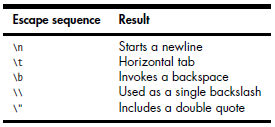
\includegraphics[width=6cm]{Screenshot_3}
%\end{figure}
%
%
%\end{frame}
%
%
%
%\begin{frame}[fragile] %%%%%%%%%%%%%%%%%%%%%%% FRAME %%%%%%%%%%%%%%%%%%%%%%%%%%%%
%
%\begin{flushleft}Examples:\end{flushleft}
%
%\begin{verbatim}
%> cat("here is a string\nsplit\tto neww\b\n\n\tlines")
%here is a string
%split	  to neww
%
%	        lines
%
%> cat("I really want a backslash: \\\nand a double 
%quote: \"")
%I really want a backslash: \
%and a double quote: "
%\end{verbatim}
%
%
%\end{frame}
%
%
%
%\begin{frame}[fragile] %%%%%%%%%%%%%%%%%%%%%%% FRAME %%%%%%%%%%%%%%%%%%%%%%%%%%%%
%
%\begin{flushleft} The function \textit{substr} takes a string x and extracts the part of the string between two character positions (inclusive),\end{flushleft}
%
%\begin{verbatim}
%> foo <- "This is a character string!"
%> substr(x=foo,start=21,stop=27)
%[1] "string!"
%
%> substr(x=foo,start=1,stop=4) <- "Here" #replace a word
%> foo
%[1] "Here is a character string!"
%\end{verbatim}
%
%
%\end{frame}
%
%
%
%\begin{frame}[fragile] %%%%%%%%%%%%%%%%%%%%%%% FRAME %%%%%%%%%%%%%%%%%%%%%%%%%%%%
%
%\begin{flushleft} The \textit{sub} function replace the first instance of a substring, while \textit{gsub} function replaces every instance of pattern.\end{flushleft}
%
%\begin{verbatim}
%> bar <- "How much wood could a woodchuck chuck"
%> sub(pattern="chuck",replacement="hurl",x=bar)
%[1] "How much wood could a woodhurl chuck"
%> gsub(pattern="chuck",replacement="hurl",x=bar)
%[1] "How much wood could a woodhurl hurl"
%\end{verbatim}
%
%
%\end{frame}

%\begin{frame}[fragile] %%%%%%%%%%%%%%%%%%%%%%% FRAME %%%%%%%%%%%%%%%%%%%%%%%%%%%%
%
%\begin{flushleft} Let's create the dataset: \end{flushleft}
%
%\begin{verbatim}
%> firstname <- c("Liz","Jolene","Susan","Boris",
%"Rochelle","Tim","Simon","Amy")
%
%> sex.num <- c(0,0,0,1,0,1,1,0)
%
%> sex.char <- c("female","female","female","male","female",
%"male","male","female")
%
%
%> mob <- c("Apr","Jan","Dec","Sep","Nov","Jul","Jul",
%"Jun")
%[1] "Apr" "Jan" "Dec" "Sep" "Nov" "Jul" "Jul" "Jun"
%\end{verbatim}
%
%
%\end{frame}



%\begin{frame}[fragile] %%%%%%%%%%%%%%%%%%%%%%% FRAME %%%%%%%%%%%%%%%%%%%%%%%%%%%%
%
%\begin{flushleft} Encode a vector as a \textit{factor} (convert \textit{integers} or \textit{characters} to \textit{factors}. \textit{Factors} can be used in statistical modeling.)\end{flushleft}
%
%\begin{verbatim}
%> sex.num.fac <- factor(x=sex.num)
%> sex.num.fac
%[1] 0 0 0 1 0 1 1 0
%Levels: 0 1
%> sex.char.fac <- factor(x=sex.char)
%> sex.char.fac
%[1] female female female male female male male female
%Levels: female male
%
%\end{verbatim}
%
%
%\end{frame}




\end{document}




